\problemname{Big City}

The participants in the Swedish Programming Olympiad love geometry, and rightfully so. The biggest
favorite among the geometries is the so-called \emph{Manhattan geometry}. The Manhattan distance
between two points \textbf{P} and \textbf{Q} in a regular grid describes how many points
you must pass to get from \textbf{P} to \textbf{Q}, given that you may only move
horizontally and vertically.

If \textbf{P} $= (x_1,y_1)$ and \textbf{Q} $= (x_2,y_2)$, then the Manhattan distance between the
points is computed as $|x_1-x_2| + |y_1-y_2|$. $|a|$ denotes the absolute value of the number $a$, i.e. we
ignore the minus sign if the number is negative.

Now it is time for you to show how much you love geometry. You are planning your move to
a big city where Manhattan distances apply. You have $N$ friends who live in the big city, but
you only have $M$ apartments to choose from. Your task is to figure out how to choose an apartment
so that the sum of the Manhattan distances to all your $N$ friends from your apartment is \emph{as small as possible}.

\begin{figure}[!h]
	\begin{center}
	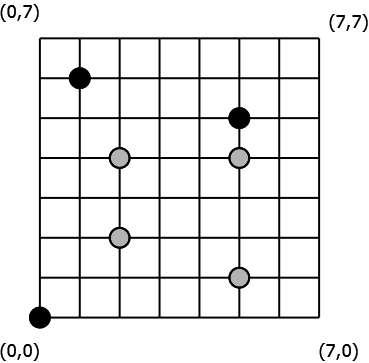
\includegraphics[scale=0.4]{Storstad}
	\end{center}
	\caption{The black dots represent apartments we can choose in the big city, and the gray dots mark where our friends live. If we choose the apartment at (0,0), the sum of distances to the friends becomes 4+6+6+9=25. If we choose the apartment at (1,6), the sum of distances becomes 3+5+6+9=23. If we choose the last apartment, the sum of distances becomes 1+4+6+4=15, and choosing the apartment at (5,5) is then optimal.}
	\label{fig1}
\end{figure}

\section*{Input}
The first line of input contains two integers $N$ and $M$ ($1 \leq N \leq 10^5$, $1 \leq M \leq 10^5$), the number of friends
and the number of apartments you can choose from.

Then follow $N$ lines with pairs of integers $x_i$ and $y_i$ ($-10\,000 \leq x_i, y_i \leq 10\,000$), describing at
which intersections in the city your friends live.

Finally follow $M$ lines with pairs of integers $x_i$ and $y_i$ ($-10\,000 \leq x_i, y_i \leq 10\,000$),
describing at which intersections in the city you can choose to live.
Note that there can be multi-story buildings in the big city (a point can appear multiple times in the input).

\section*{Output}
Output an integer: the smallest possible sum of Manhattan distances to your $N$ friends from your apartment.

Note that the answer does not always fit in a $32$-bit integer.

\section*{Scoring}
Your solution will be tested on a set of test groups.
To earn points for a group, you must pass all test cases in that group.

\noindent
\begin{tabular}{| l | l | p{12cm} |}
  \hline
  \textbf{Group} & \textbf{Points} & \textbf{Constraints} \\ \hline
  $1$   & $40$       & $N \leq 10^4$ and $M \leq 100$ \\ \hline
  $2$   & $60$       & No additional constraints.\\ \hline
\end{tabular}
